\documentclass[12pt,a4paper,english]{article}


% adding the line below for Multifile document support with LatexTools Sublime package 
%!TEX root = manuscript.tex


\usepackage[utf8]{inputenc}
\usepackage[english]{babel}

% Quotes 
\usepackage[square]{natbib}
\bibliographystyle{abbrvnat}

% For hyperlinks in the pdf 
\usepackage{hyperref}

% Glossaries
%\usepackage[acronym]{glossaries}
\usepackage[acronym,shortcuts]{glossaries}

% Font Helvetica
\renewcommand{\familydefault}{\sfdefault}
\usepackage[T1]{fontenc}

% Margins
\usepackage{geometry}
 \geometry{
 a4paper,
 total={170mm,257mm},
 left=20mm,
 top=20mm,
 }

% Linespace
\linespread{1.5}

% For pictures in the pdf
\usepackage{graphicx}

% For tables
\usepackage{multirow}
\usepackage{booktabs}
\usepackage{threeparttable}

% For ref with figure, table or equation before the number
\usepackage{cleveref}

% landscape page
\usepackage{lscape}

% for argmin and argmax
\usepackage{amsmath}
\DeclareMathOperator*{\argmin}{argmin}

% Glossary 
\usepackage[acronym]{glossaries}
%\makeglossaries

% Captions
\usepackage{booktabs,caption}

% Color
\usepackage{xcolor}

% Cross out words
\usepackage[normalem]{ulem}

% This is for me to comment

% Not using the pdfcomment package but it is an interesting one  
%\usepackage[author={Louis Mayaud}]{pdfcomment}

% Select what to do with todonotes: 
% \usepackage[disable]{todonotes} % notes not showed
\usepackage[draft]{todonotes}   % notes showed

% Select what to do with command \comment:  
% \newcommand{\comment}[1]{}  %comment not showed
\newcommand{\comment}[1]
{\par {\bfseries \color{blue} #1 \par}} %comment showed

\makeglossaries

\newacronym{adhd}{ADHD}{Attention Deficit/Hyperactivity Disorder}
\newacronym{nfb}{NFB}{neurofeedback}
\newacronym{eeg}{EEG}{electroencephalogram}
\newacronym{smr}{SMR}{Sensorimotor Rhythm}
\newacronym{mri}{MRI}{Magnetic Resonance Imagery}
\newacronym{tbr}{TBR}{Theta Beta Ratio}
\newacronym{scp}{SCP}{Slow Cortical Potential}
\newacronym{erp}{ERP}{Event-Related Potential}
\newacronym{rct}{RCT}{Randomized Controlled Trial}
\newacronym{hkd}{HKD}{Hyperkinetic Disorder}
\newacronym{es}{ES}{Effect Size}
\newacronym[plural=SEs, firstplural=Summary Effects]{se}{SE}{Summary Effect}
\newacronym{irb}{IRB}{Institutional Review Board}
\newacronym{ols}{OLS}{Ordinary Least Squares}
\newacronym{wls}{WLS}{Weighted Least Squares}
\newacronym{wrss}{WRSS}{Weighted Residual Sum of Squares}
\newacronym{lasso}{LASSO}{Least Absolute Shrinkage and Selection Operator}
\newacronym{pblind}{PBLIND}{Probably Blind}
\newacronym{mprox}{MPROX}{Most Proximal}
\newacronym{eog}{EOG}{Electro-Oculogram}
\newacronym{mse}{MSE}{Mean Square Error}
\newacronym{tova}{TOVA}{Test of Variables of Attention}
\newacronym{cpt}{CPT}{Continuous Performance Test}
\newacronym{sart}{SART}{Sustained Attention to Response Task}
\newacronym{fmri}{fMRI}{functional Magnetic Resonance Imaging}
\newacronym{pet}{PET}{Positron Emission Tomography}
\newacronym{saob}{SAOB}{Systematic Analysis of Biases}
\newacronym{agcl}{AgCl}{Silver Chloride}
\newacronym{au}{Au}{Gold}
\newacronym{emg}{EMG}{Electromyogram}
\newacronym{iapf}{iAPF}{individual Alpha Peak Frequency}



\begin{document}

% adding the line below for Multifile document support with LatexTools Sublime package 
%!TEX root = manuscript.tex

% Title

\title{Neurofeedback on children with Attention-Deficit/Hyperactivity Disorder: what factors influence its efficacy?} % Article title
\maketitle
Aurore Bussalb$^a$, Richard Delorme$^b$, Eric Acquaviva$^b$, Marco Congedo$^c$, Jean-Arthur Micoulaud-Franchi$^d$, Louis Mayaud$^a$ 
\smallbreak
\noindent $^a$: Mensia Technolgies, Paris France \\
\noindent $^b$: Hôpital Robert Debré, Paris France \\ % à compléter plus précisément
\noindent $^c$: GIPSA-Lab, Grenoble France \\
\noindent $^d$: Univ. Bordeaux, SANPSY, USR 3413, F-33000 Bordeaux, France 
\smallbreak
\noindent\textbf{Full postal address} \\
Mensia Technologies \\
Plateforme d'innovation Boucicaut \\
130 rue de Lourmel \\
75015 Paris - France \\
Aurore Bussalb's e-mail: aurore.bussalb@mensiatech.com \\
Louis Mayaud's e-mail: lm@mensiatech.com 

\clearpage

\begin{abstract}
% adding the line below for Multifile document support with LatexTools Sublime package 
%!TEX root = manuscript.tex

% Abstract

\noindent Numerous trials and several meta-analysis have been published on the efficacy of 
the Neurofeedback (NFB) treatment for Attention Deficit Hyperactivity Disorder (ADHD) in children 
and adolescents, showing inconsistent findings. This work replicates and extents the last meta-analysis 
published on this subject \citep{Cortese2016} by adding two randomized control trials (RCTs) that have been published since.
We also perform a systematic analysis of biases (SAOB), which takes advantage
of the technical and methodological heterogeneity of the studies included in the meta-analyses
rather than suffering from it.
The SAOB was performed on k = 31 trials meeting the same inclusion criteria as the earlier meta-analysis 
(but the requirement for a control arm). Our extended meta-analysis confirmed the results previously obtained: effect
sizes were significant when clinical scales of ADHD were rated by parents (non-blind, p-value = 0.0017), but not when rated by 
teachers (considered as probably blind, p-value = 0.14). The effect size was significant according to both raters for 
the subset of studies meeting the definition of "standard NFB protocols" (parents p-value = 0.0054; teachers p-value = 0.043, 
k = 4 studies). The SAOB identified three main factors that might have an impact on NFB efficacy: first, a more intensive treatment, but
not treatment duration, was associated with higher efficacy; second, high-quality EEG systems improved the effectiveness of the NFB 
treatment; third, teachers reported a lower improvement as compared to parents. In addition, to all raw data we used (31 studies), 
we release a complete Python library for performing meta-analysis, for easing the replication of this and previous studies as well 
as for future projects. In conclusion, more than replicating previous findings, we introduced here a new way to look into the 
heterogeneity of clinical trials.

% frontiers: 350

\vskip 0.2in
\noindent keywords: ADHD, Neurofeedback, influencing factors, analysis of bias, linear regression, decision tree, meta-analysis.
\end{abstract}

% adding the line below for Multifile document support with LatexTools Sublime package 
%!TEX root = manuscript.tex

% Introduction

\section{Introduction} 

% What is ADHD? What are its consequences?
\glsfirst{adhd} is a common child psychiatric disorder characterized by impaired attention and/or hyperactivity/impulsivity.
Symptoms may persist in adulthood with clinical significance, which makes \gls{adhd} a life-long problem for many
patients \citep{Faraone2006}. The prevalence of \gls{adhd} is about 5\% in school-aged children yielding to an estimated
2.5 millions of children in Europe \citep{DSM-5}. \gls{adhd} impacts children's well-being with many of them suffering
from low self esteem \citep{Shaw2005} and underachieving at school \citep{Barry2002}. Parents are equally affected by this
situation since child's behavior is commonly attributed to bad parenting \citep{Harpin2005}. From a societal point
of view, \gls{adhd} has a high financial impact: a survey of 2013 in Europe estimated at between $9,860$ and 
$14,483$ Euros per patient/year the cost related to \gls{adhd} \citep{le2014}. 

% How is it diagnosed?
The diagnosis of \gls{adhd} primarily relies on questionnaire-based clinical evaluation \citep{DSM-5}, which can be
supported with objective assessment metrics of executive function such as the \gls{tova} \citep{Forbes1998}, the
\gls{cpt} \citep{Barkley1991}, and the \gls{sart} \citep{Robertson1997}. Objective markers of brain function
using \gls{eeg}, \gls{fmri}, or \gls{pet} are not considered useful to improve diagnosis at the individual
level \citep{Neba}, but can help differentiating groups of patients \citep{Johnstone2005}.  
In particular, different phenotypes of \gls{adhd} patients present with an increase in the \gls{eeg} theta waves 
power (4-8Hz) and/or a decrease of \gls{eeg} beta waves power (12-32Hz) in frontal areas, or a decrease in the \gls{eeg} 
\gls{smr} power (13-15Hz) in the central area \citep{Monastra2005, Matouvsek1984, Janzen1995, loo2017}.  

% How is it treated? 
Among all existing treatments, the most widely used is psychostimulants, which have been proven to be efficacious
\citep{Taylor2014, Storebo2015}. However, their long-term effectiveness and side effects are still debated and form 
an active area of research \citep{DuPaul1998, Swanson2001, Jensen1999}. Moreover, \gls{adhd} children under medication 
commonly suffer from mild side effects such as loss of appetite and sleep disturbance, however serious adverse events
are rare \citep{Storebo2015, Cooper2011}. These drawbacks make some parents and clinicians reluctant to 
opt for such treatment, turning them to non-pharmaceutical alternatives such as dietary changes \citep{Belanger2009} and behavioral 
therapy, which have been proven to be less efficacious \citep{Sonuga-Barke2013}.

% What is NFB? 
\glsfirst{nfb} is another non-pharmaceutical and non-invasive approach aiming at the reduction of \gls{adhd} symptoms 
\citep{Arns2015, Steffert2010, Marzbani2016}. Shortly after the discovery of the brain's electric activity by 
\citet{Berger1929}, \citet{Durup1935} proved it could be voluntarily modulated leading to a series of finding on the 
self-regulation of brain activity. The first indication of the therapeutic potential of brain activity operant-conditioning 
came forty years later when \citet{Sterman1974} serendipitously found that training the \gls{smr} activity reduces the incidence 
of epileptic crisis in kerozen-exposed cats. The technique, then known as \gls{nfb}, quickly became investigated in various 
fields of neuropsychiatry including, most notably, \gls{adhd} \citep{Lubar1976, Rossiter1995, Linden1996, Maurizio2014}.

Thus, \gls{nfb} is a self-paced brain neuromodulation technique that represents one's brain activity in real-time using auditory 
or visual modulations, on which learning paradigms, such as operant conditioning
\citep{Reynolds1975} or voluntary control, can be applied. To deliver this intervention, neurophysiological time series 
analyzed in real-time so as to be incorporated in feedback applications such as serious games leveraging learning paradigms \citep{Wang2010}. 
These data represent the activity of a population of neurons involved in attentional networks, which is translated into 
visual or auditory cues. The sensory feedback constitutes the rewards mechanism promoting learning using operant conditioning 
protocol \citep{Sherlin2011}. Operant conditioning enables neural plasticity supporting the child in the task repetition \citep{Skinner1961}, 
which is supposed to result in long-lasting neuronal reorganization \citep{VanDoren2017}. 

Several \gls{nfb} protocols have been proposed and investigated to decrease the symptoms of \gls{adhd}:
\begin{itemize} 
  \item protocols based on neural oscillations, using frequency-band power training: enhance \gls{smr} \citep{Beauregard2006}, reduce theta 
	  or enhance beta, or a composite protocol as enhancing beta while suppressing theta, also known as the \gls{tbr}
    protocol \citep{Lubar1976, Arns2013}; 
  \item the protocol based on the \glspl{scp} training consisting in the regulation of
    cortical excitation thresholds by focusing on activity generated by external cues 
    \citep{Heinrich2004, Banaschewski2007}; 
  \item the protocol to enhance \glspl{erp}: P300 amplitude can be considered as a specific
    neurophysiological marker of selective attention \citep{Fouillen2017}.  
\end{itemize} 

% Clinical evidence of NFB
\gls{nfb} efficacy on the core symptoms of \gls{adhd} (inattention, hyperactivity, and impulsivity) has been the 
subject of several meta-analytic studies \citep{Loo2005, Lofthouse2012, Arns2009, Micoulaud2014, Sonuga-Barke2013}. 
\textcolor{red}{These studies don't reach a consensus on the efficacy of \gls{nfb}: although \citet{Arns2009} and \citet{Micoulaud2014} 
find results in favor of its efficacy, especially on the inattention component as highlighted by \citeauthor{Micoulaud2014}, \citet{Loo2005, 
Lofthouse2012, Sonuga-Barke2013} voice their reserves and ask for better evidence from blinded assessment.}

% Position of the problem
\textcolor{red}{The last meta-analysis addressing the efficacy of \gls{nfb} has been published by \citet{Cortese2016}, including a total of 13
\glspl{rct}. The results of this analysis are mixed: when based on parent assessments, which are not blind to treatment, they are significantly 
in favor of \gls{nfb} whereas when the evolution of symptoms is rated by teachers (considered as probably blind), results are no longer 
significant. Thus, the authors called for better evidence from blinded assessments in order to support \gls{nfb} as a treatment for \gls{adhd} symptoms.
However, some choices made in this meta-analysis, which might have an impact on the results, have since been debated by the community}. Specifically, 
\citet{Micoulaud2016} criticized the use of an uncommon behavioral scale provided by \citet{Steiner2014} for the teachers' assessments 
and the inclusion of a pilot study carried out by \citet{Arnold2014}. 

% Work done here
Finally, because of the publication of new \glspl{rct} meeting \citeauthor{Cortese2016}'s inclusion criteria, we
decided to update the meta-analysis and take the opportunity to investigate the impact of the controversial choices.
\textcolor{red}{While performing it, we realized that this approach presents some loopholes: first, assuming that the difference between teacher and parent
assessments can solely be explained by placebo effect; second, pooling together heterogeneous studies in terms of methodology and technical
implementation. An interesting approach, but not commonly performed, to assess the \gls{nfb} efficacy would be to analyze the specificity of the \gls{eeg} changes with respect 
to trained neuromarkers \citep{Maurizio2014}. In our case, based on the data to our disposal, we take advantage of the technical and methodological heterogeneity 
of the \gls{nfb} trials rather than suffering from it, by extending the present work with a novel method, the \glsfirst{saob}.} Indeed, the \gls{nfb} domain is 
characterized by a clinical literature that is tremendously heterogeneous: studies differ methodologically (random assignment and 
presence of a blind assessment for instance), in the \gls{nfb} implementation (number of sessions, session and treatment length,
and type of protocol for instance) as well as on the acquisition and processing of the \gls{eeg} signal. \textcolor{red}{Description and analysis of different types 
of \gls{nfb} implementation was subject to several studies \citep{Arns2014, Enriquez2017, Vernon2004, Jeunet2018} but to our knowledge none used statistical 
tools to quantify their influence on clinical endpoints.}

Since methodological and technical implementations of studies are very likely to influence their outcomes \citep{Congedo2004}, we suggest 
here to identify which of the factors independently influence the clinical efficacy with the use of appropriate statistical tools. 
\textcolor{red}{In addition, to all raw data we used, a complete Python library is released for performing meta-analysis, for easing the replication of 
this and previous studies as well as for future projects.}


% number of words: 835






% adding the line below for Multifile document support with LatexTools Sublime package 
%!TEX root = manuscript.tex

% Materials and Methods

\section{Materials and Methods}

\subsection{Inclusion criteria}

Search terms were directly taken from \citet{Cortese2016} with the exception of the need for a control arm, 
which is detailed in Supplemental Materials \citep{Supplementalmaterial}. The requirements included:
\begin{itemize}
	\item studies have to assess \gls{nfb} efficacy; 
	\item subjects must have received a diagnosis of \gls{adhd} based on DSM-IV \citep{DSM-4}, DSM-5 \citep{DSM-5}, 
	ICD-10 \citep{ICD101993} criteria, or by a qualified psychiatrist; 
	\item studies have to be written in English, German, Spanish, or French;
	\item studies have to include at least eight subjects in each group;
	\item patients must be younger than 25 years old;
  \item the publication has to disclose sufficient details about the data
	to compute required metrics for the ensuing analysis.
\end{itemize} 
The studies satisfying all these criteria were included in the \gls{saob}.
In order to replicate and update \citeauthor{Cortese2016}'s meta-analysis, we applied the original inclusion criteria of 
their meta-analysis to our search (the main difference being the presence of a control group). 

\subsection{Outcome definition} 

In the included studies, the severity of \gls{adhd} symptoms have been assessed by parents and, whenever available, 
by teachers. \citet{Cortese2016} and \citet{Micoulaud2014} defined parents as \gls{mprox} raters who were 
not blind to the treatment, as opposed to teachers, who were considered as \gls{pblind} raters. 
This distinction is intended to assess the amplitude of the placebo effect, where it is hypothesized that teachers, 
who are presumed to be more blind to the intervention, are less influenced in their assessment. 
Efficacy of \gls{nfb} was measured using clinical scales, such as the \gls{adhd}-RS \citep{Pappas2006}, 
on the following outcomes: inattention, hyperactivity/impulsivity, and total scores. The factor analysis was 
performed using the total score.

\subsection{Meta-analysis}

The goal of a meta-analysis is to aggregate results from different clinical investigations and offer a 
consolidated body of evidence. To achieve this, it is necessary to assume 
some level of homogeneity in the design of the studies: inclusion criteria, and the presence and type of control 
(active, semi-active, or non-active). Because studies occasionally 
use slight variations of a clinical scale and because of the clinical heterogeneity of patients and control, 
the scores are standardized before being pooled into a \gls{se}. The between-\gls{es} is one such standardized metric, 
which we have implemented in this paper (see Supplemental Materials \citep{Supplementalmaterial}). 

The meta-analysis was performed with a Python package developed for this work. The package offers a transparent 
approach for the choice of parameters in an effort to ease replicability. We have benchmarked it against RevMan version 5.1 
\citep[UK, London]{RevMan} by replicating \citet{Cortese2016}'s work. 
The code is made fully available on a GitHub repository \citep{Bussalb2019}, together with all the \glspl{rct} raw data we have used
in the present study.
 
Before updating the \citet{Cortese2016} work with recently published studies
\citep{Strehl2017, Baumeister2016}, we decided to run a sensitivity analysis investigating the choices 
that later proved controversial \citep{Micoulaud2016}. The investigated changes included:
\begin{itemize}
\item the between-\gls{es} of \citeauthor{Arnold2014}'s study was computed from the post-test clinical values taken 
after the completion of the 40 sessions, in contrast to \citet{Cortese2016}'s report which used the results 
after only 12 sessions because the endpoint values were not available at the time of his study;
\item the between-\gls{es} computed from the teachers' assessment reported by \citet{Steiner2014} relied on the BOSS 
Classroom Observation \citep{Shapiro2010}. This is an atypical scale to quantify \gls{adhd} symptoms since 
the Conners Rating Scale Revised \citep{Conners1998, Christiansen2014, Bluschke2016}, a well-defined
\citep{Collett2003, Epstein2012} and broadly used metric, was available in this study. Thus, we decided 
to compute the between-\gls{es} based on the Conners-3 already used in this study to compute the 
parents' between-\gls{es}.  
\end{itemize} 

As initially suggested by \citeauthor{Cortese2016}, the analysis was run on two subgroups of studies 
with the two choices described above: one gathering studies following the standard protocol defined by 
\citet{Arns2014} and a second including only participants not taking medications during the clinical trial.

\subsection{Identify factors influencing the neurofeedback}

While revisiting the existing meta-analyses, it became apparent that the studies pooled together were highly heterogeneous 
in terms of methodological and practical implementation. For instance, all \gls{nfb} 
interventions were pooled together regardless the quality of acquisition, the quality of EEG data, and the trained 
neuromarker. Equally, the methodological implementations varied significantly, requiring the 
'subgroup' analysis (for instance, gathering studies following standard protocols) that are somewhat arbitrary. To circumvent these limitations, we 
implemented a novel approach: the \gls{saob}. With this method, the within-\gls{es} of each intervention was considered 
as a dependent variable to be explained by methodological and technical factors. Such analysis aims at identifying known methodological 
biases (e.g.\ blind assessments negatively associated 
with within-\gls{es}) and possible technical factors (e.g.\ a good control on real time data quality positively influences the 
treatment outcome). 

\subsubsection{Identify and pre-process factors}

We classified the factors influencing the efficacy of \gls{nfb} into five categories: methodological, technical,
demographics, and quality of the signal and acquisition. 
Factors were chosen based on that reported in the literature as presumed to influence \gls{es}, 
and categorized as follows:

\begin{itemize}
  \item \emph{the signal quality}: correction of ocular and generic (amplitude-based) artifacts;
  \item \emph{the population}: intake of psychostimulants during \gls{nfb} treatment and the age range of children
  included;
  \item \emph{the methodological biases}: the presence of a control group, the blindness of assessors, 
  the randomization of subjects in controlled trials, and the approval of the study by an \gls{irb};
  \item \emph{the \gls{nfb} implementation}: the protocol used (\gls{scp}, \gls{smr}, 
  theta up, beta up in central areas, theta down), the presence of a transfer phase during \gls{nfb} training, the 
	possibility to train at home or at school with a transfer card, 
  the type of thresholding for discrete reward, the number of \gls{nfb} sessions, the length and frequency of the sessions, and the length of
  the treatment;
  \item \emph{the acquisition quality}: the presence of one or more active electrodes and the \gls{eeg} data quality. 
  The latter was coded as an indicator between 1 and 3, using the following criteria:   
	\begin{description}
	  \item[\emph{the type of electrodes used}:] \gls{agcl}/Gel or \gls{au}/Gel;
    \item[\emph{the use of impedance mode}:] a quality check of electrode contacts
		ensuring an inter-electrode impedance smaller than $40k\Omega$;  
    \item[\emph{the level of hardware certificate}:] compliance with ISO-60601-2-26 \citep{ISO-60601-2-26:2012}.
	\end{description}
	A quality score equal to 3 was assigned if all the above criteria were satisfied. If at least one was satisfied
	the quality score was set to 2, otherwise the score was set to 1.
\end{itemize}	

To prevent any bias in the analysis, the names of the factors were hidden during the entire analysis so that the data scientists (AB, QB,
DO, and LM) were fully blind to them. The names were revealed only when the data analysis and results were accepted as valid: 
this included choice of variable normalization and validation of model hypothesis, as detailed below.

The pre-processing of factors for the analysis included the following steps: factors for which there were too many 
missing observations, arbitrarily set to more than 20\% of the total observations, were removed from the analysis. 
Furthermore, if a factor had more than 80\% similar observations it was also removed. Categorical variables were 
coded as dummies, i.e., the presence of the factor was represented with 1 and its absence with 0. All variables 
were standardized by subtracting the mean and then dividing by the standard deviation (not applied before the decision tree described below).

\subsubsection{Explaining within effect sizes with factors}

To compute the within-\gls{es}, the  means of total \gls{adhd} scores given by parents and teachers were used. Moreover, 
in case studies providing results for more than one behavioral scale the within-\gls{es} scores were computed for each one as 

\begin{equation*}
\label{eq:factors_effect_size_within_subject}
\text{ES} = \frac{M_{\text{post,T}} - M_{\text{pre,T}}}{\sqrt{\frac{\sigma_{\text{pre,T}}^2 + \sigma_{\text{post,T}}^2}{2}}},
\end{equation*} 
\noindent where $M_{\text{t,T}}$ is the mean of clinical scale, for treatment T, taken at time t (pre-test or post-test) and $\sigma_{\text{t,T}}$ represents 
its standard deviation. With this definition, we focus on the effect of the treatment within a group \citep{Cohen1988} as commonly reported 
in the literature \citep{Arns2009, Maurizio2014, Strehl2017}. This within-\gls{es} enables us to quantify 
the efficacy of \gls{nfb} inside the treatment group. 

The within-\gls{es} was then considered as a dependent variable to be explained by the factors (the independent variables). 
The following three methods, implemented with the Scikit-Learn Python \citep[version 0.18.1]{Pedregosa2011} and the Statsmodels Python
\citep[version 0.8.0]{Seabold2010} libraries, were used to perform the regression:
\begin{itemize}
  \item weighted multiple linear regression (\gls{wls}) \citep{Montgomery2012};
	\item sparsity-regularized linear regression with \gls{lasso} \citep{Tibshirani1996};
	\item decision tree \citep{Quinlan1986}.
\end{itemize}

The aim of the linear regression is to estimate the regression coefficients linking the factors
to the within-\gls{es}. A significant coefficient (here and hereafter meaning significantly different from zero) indicates
that the associated factor has an influence on \gls{nfb} efficacy and its sign the direction of the effect.

The \gls{wls} differs from a traditional linear regression estimated with \gls{ols} in that a weight is assigned 
to each observation in order to account for the multiplicity of reported clinical endpoints in some studies. In addition, the 
weight was also set as a function of the sample size to account for variations in sample sizes. Specifically, the weight of each study 
was taken as the ratio between the experimental group's sample size and the number of behavioral scales available.
We also ran the analysis using the \gls{ols} method to assess the impact of the weights on the results. 

The second linear method applied was the \gls{lasso}, which naturally incorporates variable selection 
into the linear model thanks to $\ell_1$-norm applied on the coefficients. A coefficient not set to zero means that 
the associated factor has an influence on \gls{nfb} efficacy and its sign indicates the direction of the effect.

The last method used to determine factors influencing \gls{nfb} was the decision tree \citep{Quinlan1986}, a hierarchical 
and non-linear method. This breaks down a dataset into smaller and smaller subsets using, at each iteration, a variable and 
a threshold chosen to optimize a simple \gls{mse} criterion \citep{James2013}. A tree is composed of several nodes and leafs, 
the importance of which decreases from the top node, called the root node, downward. 

Given that these methods are intrinsically different we compared their results. For instance, the decision
tree captures variable interactions and can relate factors to within-\gls{es} in a non-linear fashion. On the other hand, the
\gls{lasso} offers an elegant mathematical framework for variable selection. Further details are provided in the Supplemental Material
\citep{Supplementalmaterial}.


%1625














% adding the line below for Multifile document support with LatexTools Sublime package 
%!TEX root = manuscript.tex

% Results

\section{Results}

\subsection{Selected studies}

Search terms entered in Pubmed returned \textcolor{red}{155} results during the last check on February 12, 2018, including 22 
articles used in previous meta-analyses on \gls{nfb}. Following the selection process illustrated 
in Figure~\ref{Figure:systematic_review_workflow}, \textcolor{red}{33} studies were included in the \gls{saob} and \textcolor{red}{16} in the meta-analysis, 
as summarized in Table~\ref{Table:table_factors_analysis_meta_analysis_list_studies}. The \textcolor{red}{33} studies selected for the \gls{saob} 
followed \citeauthor{Cortese2016}'s criteria, with the exception of the requirement for a control group. 
Indeed, since within-\gls{es} were considered in this analysis, a control group was not required.

\subsection{Meta-analysis}

The replication of \citeauthor{Cortese2016}'s results obtained are presented 
in Table~\ref{Table:meta_review_comparison_revman_and_python_with_choices}:

\begin{itemize}
    \item when computing the between-\gls{es} for \citet{Arnold2014} with the values after 40 sessions of \gls{nfb}, 
      smaller between-\gls{es} were found as compared to those found by \citet{Cortese2016}, which was unexpected since  
			the clinical efficacy is supposed to increase with the number of \gls{nfb} sessions. These lower between-\gls{es}
			impacted the \gls{se}: they were slightly lower when computed with this choice although they nonetheless remained significant (see the three first lines 
			of Table~\ref{Table:meta_review_comparison_revman_and_python_with_choices});  
    \item when relying on the teachers' ratings from the Conners-3 to compute the between-\gls{es} of \citet{Steiner2014}, 
		higher \glspl{se} were found in attention but not for total and hyperactivity score. However, this different choice of 
		scale did not affect the statistical significance of the \glspl{se} (see the three last lines 
			of Table~\ref{Table:meta_review_comparison_revman_and_python_with_choices}).
\end{itemize}

The meta-analysis was then extended by adding \textcolor{red}{three} new articles \citep{Strehl2017, Baumeister2016, Bazanova2018}. 
\citet{Bazanova2018} \textcolor{red}{gave parents' assessments for all outcomes}, \citet{Baumeister2016} provided results solely for parents' 
total outcome, whereas \citet{Strehl2017} gave both teachers' and parents' assessments for all outcomes. \textcolor{red}{To be consistent 
with the \gls{saob}, only the standard \gls{nfb} group of }\citet{Bazanova2018} \textcolor{red}{was included in this update}. Despite favorable results 
for \gls{nfb}, particularly on parents' assessments, adding these \textcolor{red}{three} new studies did not change either the magnitude or the significance 
of the \gls{se}, for any outcome regardless of the raters, as illustrated in 
Figure~\ref{Figure:meta_review_forest_plots_update_meta_analysis_our_choices_no_colors_2-columns_fitting_image}. 

Regarding the "standard protocol" subgroup, \citet{Cortese2016} found all the outcomes significant except for the 
hyperactivity symptoms rated by teachers, which showed only a statistical trend (p-value = 0.11). Similar results 
were obtained when adding the most recent studies meeting this definition \citep{Strehl2017, Baumeister2016} (p-value = 0.11). 
The \gls{se} for the total outcome assessed by teachers remained significant with the addition of the new
\gls{rct} (p-value = 0.043), thus giving more strength to this result since it is now based on four studies including 283
patients in total.

As for the no-drug subgroup, \glspl{se} were found significant for the inattention symptoms assessed by parents (p-value = \textcolor{red}{0.017}). 
In addition, the differences in \citet{Arnold2014} values and the inclusion of \citet{Bazanova2018} caused a 
loss of significance in hyperactivity outcome for parents (p-value = \textcolor{red}{0.062}) compared to \citet{Cortese2016} 
(p-value = 0.016). \textcolor{red}{Only} \citet{Bazanova2018} \textcolor{red}{was included in this subgroup: in the two other 
studies the subjects were taking psychostimulants during the trial.}

All the clinical scales used to compute the between-\gls{es} following our choices are summarized in the Supplemental Materials.

\subsection{Factors influencing Neurofeedback}

This analysis was performed on \textcolor{red}{33} trials \textcolor{red}{(corresponding to 67 observations)} assessing the efficacy of \gls{nfb}, as presented 
in Table~\ref{Table:table_factors_analysis_meta_analysis_list_studies}. \textcolor{red}{The outlier rejection removed two training groups
of \citet{Bazanova2018} from the analysis because their within-\gls{es} were out of the bounds.} Among the \textcolor{red}{28} 
factors selected, \textcolor{red}{nine} were removed because there were too many missing observations or because they were too homogeneous: beta up in frontal areas, 
the use of a transfer card, the type of threshold for the discrete rewards (incremental or fixed), the \gls{eeg} quality equal of 3, the 
presence of a control group, \textcolor{red}{the individualization of the frequency bands based on the \gls{iapf}, coupling 
\gls{nfb} with \gls{emg}-Biofeedback, the severity of \gls{adhd} symptoms at baseline, and the degree of engagement with NF intervention}.  

All results are presented in Table~\ref{Table:table_factors_analysis_results_summary}. These results, require 
careful interpretation since each technique provided slightly different results. These differences 
may depend on the different assumptions of the model and several other factors. Nonetheless, we are inclined to 
trust the findings that are consistent across methods. 

The \gls{wls} technique identified \textcolor{red}{nine} significant factors for an adjusted R-squared of \textcolor{red}{0.62} (see second column of 
Table~\ref{Table:table_factors_analysis_results_summary}). 
When applying the \gls{ols}, the same factors were significant \textcolor{red}{(except the \gls{eeg} quality equal of 2 and the presence of more than one active electrode)}
with a lower adjusted R-squared \textcolor{red}{(0.35)}. The \gls{lasso} regression selected \textcolor{red}{six} significant factors (see third column of 
Table~\ref{Table:table_factors_analysis_results_summary}). With these methods, a negative coefficient means 
that the factor is in favor of the efficacy of \gls{nfb}. The decision tree is presented in Figure~\ref{Figure:factors_analysis_decision_tree_results}: 
the best predictor in our case was the \gls{pblind} (see last column of 
Table~\ref{Table:table_factors_analysis_results_summary}). \textcolor{red}{Four} other factors also split the subsets; however, 
increasingly fewer samples are available the lower we get into the tree, making the interpretation increasingly doubtful.  

Several factors were common to the three methods used. These included, in particular: the assessment 
by a blind rater, the treatment length, and an \gls{eeg} quality score equal to 2 \textcolor{red}{(see lines 1, 9, and 19 of 
Table~\ref{Table:table_factors_analysis_results_summary})}.
The methods also agreed on the direction of the effect for these factors: 
a shorter treatment and recording of the \gls{eeg} with a good-quality system appears preferable, whereas teachers' assessment appears less favorable 
compared to parents' assessment.

\textcolor{red}{It is more doubtful the influence of the factors returned by only one or two methods (see lines 2, 3, 7, 8, 11, 16, 17, and 20
of Table~\ref{Table:table_factors_analysis_results_summary}). In particular: 
\begin{itemize}
\item both \gls{wls} and \gls{lasso} found that using more than one active electrode during \gls{nfb} appears to lead to an higher efficacy;
\item both \gls{wls} and the decision tree found that performing a higher number of sessions seems to be preferable;
\item both \gls{lasso} and the decision tree found that a higher number of sessions per week appear to positively influence the efficacy of the \gls{nfb} treatment.
\end{itemize}
Five factors were returned by only one of the methods: randomizing the groups, the \gls{irb} approval, the session length, the presence of a transfer phase, 
and the correction or rejection of ocular artifacts}

\textcolor{red}{Eight factors were never selected by the three methods (see lines 4, 5, 6, 12, 13, 14, 15 and 22 of 
Table~\ref{Table:table_factors_analysis_results_summary}): the children's minimum and maximum age, being on drugs during \gls{nfb} treatment,
the protocols \gls{smr}, beta up in central areas, theta down, and \gls{scp}, and the artifact correction based on amplitude.}
Thus, these factors overwhelmingly appear not to have an influence on \gls{nfb} efficacy. 

In the next section we discuss only the factors that were selected by at least two of the three methods. 

% words number = 1081

% adding the line below for Multifile document support with LatexTools Sublime package 
%!TEX root = manuscript.tex


% Discussion

\section{Discussion}

\subsection{Meta-analysis} 

\textcolor{red}{This replication and update of a meta-analysis did not meet all PRISMA recommendations \citep{Moher2009}. In particular, the risk of bias
in individual and across studies was not assessed.}  

In the meta-analysis performed here, we challenged some choices made by \citeauthor{Cortese2016}, which proved controversial: 
the computation of between-\gls{es} based on an unusual scale \citep{Steiner2014} and the inclusion of a pilot study \citep{Arnold2014} 
whose end point values were not available at the time \citeauthor{Cortese2016} conducted his meta-analysis. We review here the 
list of changes, their justification, and their impact on the analysis.
 
First, relying on the Conners-3 \citep{Conners2011} instead of the BOSS Classroom Observation \citep{Shapiro2010} for
teachers ratings seems preferable because this scale is more commonly used \citep{Christiansen2014, Bluschke2016} and is
the revision of the Conners Rating Scale Revised \citep{Conners1998} whose reliability has been studied \citep{Collett2003}. 
However, relying on one or the other scale did not change the significance of the between-\gls{es}, regardless the outcome.

Second, to compute the between-\gls{es} of \citet{Arnold2014} the clinical scores taken when all sessions were completed were 
used instead of looking at interim results as in \citeauthor{Cortese2016}. Some studies suggested that the number of sessions 
correlates positively with the changes observed in the \gls{eeg} \citep{Vernon2004} so that a lower number of sessions would 
lead to artificially smaller between-\gls{es}. Here, the between-\gls{es} computed with the values at post test of \citet{Arnold2014} were smaller 
than those obtained after 12 sessions but these differences did not lead to a change of significance of the \gls{se}. 

To conclude on that meta-analysis, although some points from the original were controversial, the impact on the
meta-analysis were minimal and did not change the statistical significance of any outcome. 
The addition of the two new studies \citep{Strehl2017, Baumeister2016} further confirmed original results. Indeed, the
significance did not change for any outcome: the \gls{se} remained significant for \gls{mprox} raters and
non-significant for \gls{pblind}. Adding two more studies increased the significance of the sensitivity analysis ran by
\citeauthor{Cortese2016}, most notably, the \gls{se} of studies corresponding to \gls{nfb} "standard protocols" \citep{Arns2014}. 
While \citeauthor{Cortese2016} found that this subset tended to perform better, particularly on the \gls{pblind} outcome, 
adding two studies extended this result on the total clinical score as well (p-value < 0.05). Despite the obvious heterogeneity 
of the studies included in this subset (particularly in terms of protocol used), these results suggest a positive relation 
between the features of this \emph{standard} design and \gls{nfb} performance. \textcolor{red}{This result is a step forward in the demonstration 
of standard \gls{nfb} protocol efficacy for the treatment of \gls{adhd}. Yet, the  studies 
included in this subset are still highly heterogeneous (particularly in terms of protocol used), which should be accounted for.}


\subsection{Factors influencing Neurofeedback}

Description and analysis of different types of \gls{nfb} implementation was subject to several studies \citep{Arns2014, 
Enriquez2017, Vernon2004, Jeunet2018} but to our knowledge none used statistical tools to quantify their influence on
clinical endpoints. 

Surprisingly, the number of sessions factor was not found significant by any method, which was somewhat
in contradiction with existing literature. For instance, \citet{Arns2014} stated that performing less than
20 \gls{nfb} sessions led to smaller effects. Similarly, \citet{Vernon2004} observed that positive changes in the \gls{eeg}
and behavioral performance occurred after a minimum of 20 sessions. However, \citet{Enriquez2017} insisted on the fact that the number of
sessions should be chosen carefully in order to avoid "overtraining". The fact that the number of sessions was not identified as a 
positively contributing factor, might be explained by the presence of only one data point with 20 sessions or less. Possibly, 
the temporal threshold of efficacy was passed for all included studies making the identification of this factor unlikely on 
this dataset. However, regardless of its statistical significance, the coefficient found by the \gls{wls} was negative, meaning 
that, as expected, the more sessions are performed, the more efficient the \gls{nfb} tends to be. 

Interestingly, \citep{Minder2018} suggests that the subject location of the \gls{nfb} training may also be an important contributing 
factor to clinical effectiveness. However this has been challenged by a recent study \citep{Minder2018} showing that 
performing \gls{nfb} at school or at the clinic has no significant impact on treatment response. 

The type of \gls{nfb} protocol was not identified by more than one method: it did not seem to influence the \gls{nfb} results. 
This little importance granted by the methods to the \gls{nfb} protocols was somewhat lower to
expectations given the centrality of the protocols in the neurophysiological mode of action and subsequent expected impact on
therapeutic effectiveness \citep{Vernon2004}. A possible explanation for this result is that these protocols were equally 
efficacious to the populations they were offered to and thereby did not constitute a significant explanatory factor. 
This result, however, does not preclude a combined and personalized strategy (offering personalized protocols based on phenotypes)
to further improve performance, as previously suggested by \citet{Alkoby2017}.

Several factors were selected by all three methods with the same direction of influence: the EEG quality, the treatment 
length, and the rater's probably blindness to the treatment. First, our analysis pointed out the fact that recording \gls{eeg} 
in good conditions leads to better results.
This can be explained by the fact that better signal quality enables to extract the \gls{eeg} patterns
linked to \gls{adhd} more correctly and henceforth leads to better learning and therapeutic efficacy \citep{Congedo2004}. 
However, it remains difficult to assess the quality of \gls{eeg} hardware (such as the amplifier used) 
because little information is provided in these studies.  
This calls for a greater care in the future studies, which should strive and to assess and report the quality of the data.

Next, it appears here that the longer the treatment, the less efficient it becomes. Arguably, the treatment length is a
proxy for treatment intensity, suggesting that a shorter treatment is more likely to succeed because the frequency of the sessions
is higher. This hypothesis was back-up by the fact that the variable \emph{session pace} (number of
sessions per week) is also associated with larger within-\gls{es} according to the \gls{wls} and \gls{lasso}. Impact of the
intensity of treatment have been investigated by \citep{Rogala2016} on healthy adults: it was observed that studies with
at least four training sessions completed on consecutive days were all successful. Overall these results suggest to adopt a high session pace, 
which is not common knowledge in the domain.

\textcolor{red}{This strongly support the effectiveness of \gls{nfb} for the treatment of \gls{adhd}. However, as expected, the assessment of symptoms by non-blind raters 
leads to far more favorable results than by \gls{pblind} raters - result widely expected and in close compliance with existing 
meta-analysis \citep{Cortese2016, Micoulaud2014}. This observation contrasts with this result and certainly would be contradictory should teachers’ 
assessments reflect some placebo effect, which has long been documented in the literature \citep{Sollie2013, Narad2015, Minder2018}. 
This discrepancy was investigated more thoroughly in the next section.}

\subsection{Analysis on the probably blind raters}

Teachers were considered as \gls{pblind} raters by \citeauthor{Cortese2016} and \citeauthor{Micoulaud2014}.
Unexpectedly, the data provided did not exactly matched the widely accepted hypothesis stating that the difference between
\gls{mprox} and \gls{pblind} can solely be explained by the placebo effect. 
Nonetheless, the stress put on \emph{probably} indicated that teachers may be aware of the treatment followed. 
An element that corroborates this hypothesis is the fact that for all the studies included in this work the amplitude 
of the clinical scale at baseline suggests that teachers did not capture the full extent of the symptoms or, said differently, 
that they were more blind to the symptoms than to the intervention as illustrated 
in Figure~\ref{Figure:discussion_on_placebo_effect_colors_2-columns_fitting_image}. 
\textcolor{red}{Indeed, before the intervention, teachers rated less severely the symptoms compared to parents and observed mostly less improvement at post-test: 
this tends to correspond more to the case A with no placebo effect than the case B}. The expected differences of ratings between 
teachers and parents have been extensively studied \citep{Sollie2013, Narad2015, Minder2018}, noting that teachers are more 
likely to underrate a child's symptom severity, especially so for younger children. As a consequence, teachers might just be less likely 
to observe a clinical change over the course of the treatment \citep{Sollie2013, Narad2015, Minder2018}. Besides, it is also clear 
that there is more variability in teachers' scores compared to parents', which could partly explain the lower \gls{es} obtained for 
\gls{pblind} raters, since the variability deflates the \gls{es}. In conclusion, using \gls{pblind} as an estimate for correcting the 
placebo effect does not appear an adequate choice. 

Another way to highlight a possible placebo effect is to focus on the decision tree illustrated in Figure
~\ref{Figure:factors_analysis_decision_tree_results}, whose results provide a good insight to comment on this.
The top node splits: on one hand 45 observations corresponding to \gls{mprox} raters and, on the other hand, 
21 observations corresponding to \gls{pblind}. If the differences observed between \gls{pblind} and \gls{mprox} raters were 
due to the placebo effect, one would expect to find in the \gls{mprox} sub-tree some factors linked to the perception
of the implication in the treatment. It was, indeed the case: session and treatment length were found significant but not in the
direction corroborating the hypothesis that they are as part of a placebo effect. Indeed, one would expect that the
longer the session and the treatment, the higher the placebo effect and the larger the within-\gls{es}. Instead, the opposite was found, 
somewhat invalidating the hypothesis. 

These results altogether suggest that \gls{pblind} assessments could hardly be used to assess placebo effect as they seem to be blinder 
to symptoms than to intervention. In the absence of ethically \citep{Holtmann2014} and technically \citep{Birbaumer1991} feasible sham 
for \gls{nfb} protocols \citep{World-Medical-Association2000}, it is necessary to fall back on acceptable methodological alternative for 
the demonstration of clinical effectiveness. Among those are the analysis of neuromarkers collected during \gls{nfb} treatment demonstrating 
that patients do \emph{control} the trained neuromarkers; that they \emph{learn} (reinforce control over time), and that these possibly 
lead to lasting brain reorganization (e.g., changes in their baseline resting state activity). The specificity of these changes, in relation 
to, which neuromarkers were trained and to the clinical improvement will be an essential component of this demonstration.  

% words number = 1506

% adding the line below for Multifile document support with LatexTools Sublime package 
%!TEX root = manuscript.tex

% conclusion

\section{Conclusion}

This work confirms \citet{Cortese2016}'s findings in the light of recent published clinical work.
In particular, studies following a standard protocol as defined by \citet{Arns2014} show significant 
clinical improvements on \gls{pblind} raters (k = 4 studies instead of 3 \citet{Cortese2016}).

Besides this meta-analysis, a new method is suggested to tackle the high heterogeneity of clinical data 
available on \gls{nfb}. This method aims at identifying factors as positively or negatively contributing 
to \gls{nfb} efficacy. Three factors were consistently found to statistically significantly explain clinical 
within-\gls{es}. First, the quality of acquisition of the \gls{eeg} was positively correlated with clinical 
efficacy. It confirms a mode of action through specific \gls{eeg} training. Likewise, treatment intensity was 
found to contribute, corroborating what is known of learning theory (memory consolidation) \citep{Mowrer1960}, 
that is a more intense treatment leads to an increased clinical efficacy. Finally, results show that the therapeutic 
efficacy measured by teachers is reduced compared to that measured by parents. This result has long been documented 
and it is widely accepted that this difference is solely imputable to the amplitude of placebo effect in \gls{nfb}. 
However, the data presented in this article tend to refute this hypothesis and suggest that teachers are simply 
exposed to less symptoms, in line with the most recent work on the topic. As a consequence, using \gls{pblind} 
endpoints to address the specificity of the clinical efficacy is not recommended and the community should instead 
rely on other available methodological tools. Those include sham \gls{nfb} and neuromarker analysis investigating 
the specificity of the \gls{eeg} changes with respect to trained neuromarkers and changes in clinical endpoints.

These elements converge to the conclusion that existing methodologies traditionally used to assess drug treatments 
in neuropsychiatric conditions may not be fully fit to the evaluation of medical devices. The series of results presented 
here however suggest the presence of a genuine signal in favor of the therapeutic efficacy of \gls{nfb}. A signal that 
should nonetheless be strengthen using the aforementioned methodological tools, neuromarker analysis in the first place.

This work also offers an open source tool for running meta-analysis and \gls{saob}: the code and data used are available, 
assuring the transparency and replicability of these analysis. 

% 357
% 241

% discolsure statement 

\section*{Conflict of Interest Statement}
A. Bussalb, Q. Barthelemy, D. Ojeda, and L. Mayaud work for Mensia Technologies.
M. Congedo served as an advisor for Mensia Technologies when this work was conducted.  

\section*{Author Contributions}
AB extracted all data from articles and performed the analysis, MC provided useful advice 
concerning statistics and the methods used, RD and EA followed closely the evolution of 
the work and provided good ideas especially on the clinical level. QB and DO gave useful 
ideas to optimally apply methods used in the \gls{saob} and helped in the interpretation 
of the results. LM oversaw all this work. 

\section*{Funding}
This research was conducted as part of a PhD thesis funded by Mensia Technologies, the 
Association Nationale Recherche et Technologie (ANRT), and the EU H2020 NEWROFEED grant.


% ACKNOWLEDGEMENTS

\section*{Acknowledgments}

We would like to thank Jean-Arthur Micoulaud-Franchi, MD, PhD for his helpful 
comments and ideas on that work. We also would to thank the Association Nationale 
Recherche et Technologie (ANRT) that partly funded this thesis as well as the EU 
H2020 NEWROFEED grant.

% 43

\section*{List of abbreviations} 
ADHD: Attention deficit/hyperactivity disorder,
NFB: Neurofeedback,
EEG: Electroencephalogram,
SMR: Sensorimotor Rhythm,
MRI: Magnetic Resonance Imagery,
TBR: Theta Beta Ratio,
SCP: Slow Cortical Potential,
ERP: Event-Related Potential,
RCT: Randomized Controlled Trial,
HKD: Hyperkinetic Disorder,
ES: Effect Size,
SE: Summary Effect,
IRB: Institutional Review Board,
OLS: Ordinary Least Squares,
WLS: Weighted Least Squares,
WRSS: Weighted Residual Sum of Squares,
LASSO: Least Absolute Shrinkage and Selection Operator,
PBLIND: Probably Blind,
MPROX: Most Proximal,
EOG: Electro-Oculogram,
MSE: Mean Square Error,
TOVA: Test of Variables of Attention,
CPT: Continuous Performance Test,
SART: Sustained Attention to Response Task,
fMRI: functional Magnetic Resonance Imaging,
PET: Positron Emission Tomography,
SAOB: Systematic Analysis of Biases,
AgCl: Silver Chloride,
Au: Gold,
EMG: Electromyogram 

\clearpage

\bibliography{bibliography}

\clearpage

\section*{Figure captions}

\begin{figure}[h!]
  \centering
	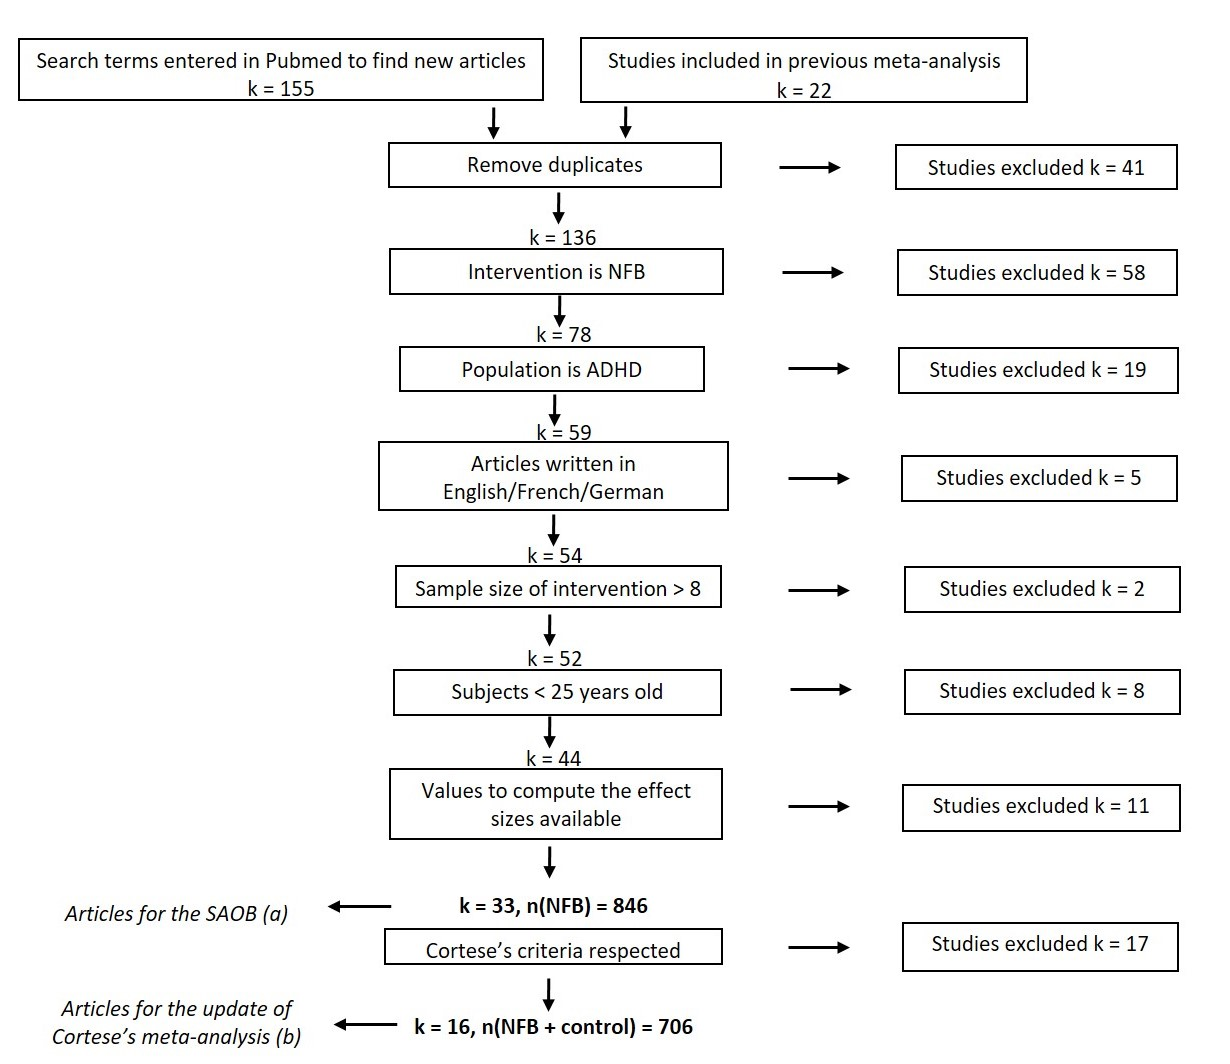
\includegraphics[width=1.0\linewidth]{figures/meta_review_factors_analysis_how_studies_are_included_no_colors_2-columns_fitting_ima.jpg} 
  \caption{Flow diagram of selection of studies (last search on December 14, 2017).  
	The subset (a) corresponds to the \citeauthor{Cortese2016}'s inclusion criteria without the requirement for the presence of a control group. The number
	of patients is only equal to the subjects in the \gls{nfb} groups.
	The subset (b) exactly corresponds to the studies included in \citet{Cortese2016} and more recent work meeting the same criteria. Here, the number of patients includes all patients
	whatever their treatment group.}
  \label{Figure:systematic_review_workflow}
\end{figure}

\begin{figure}[h!]
  \centering
  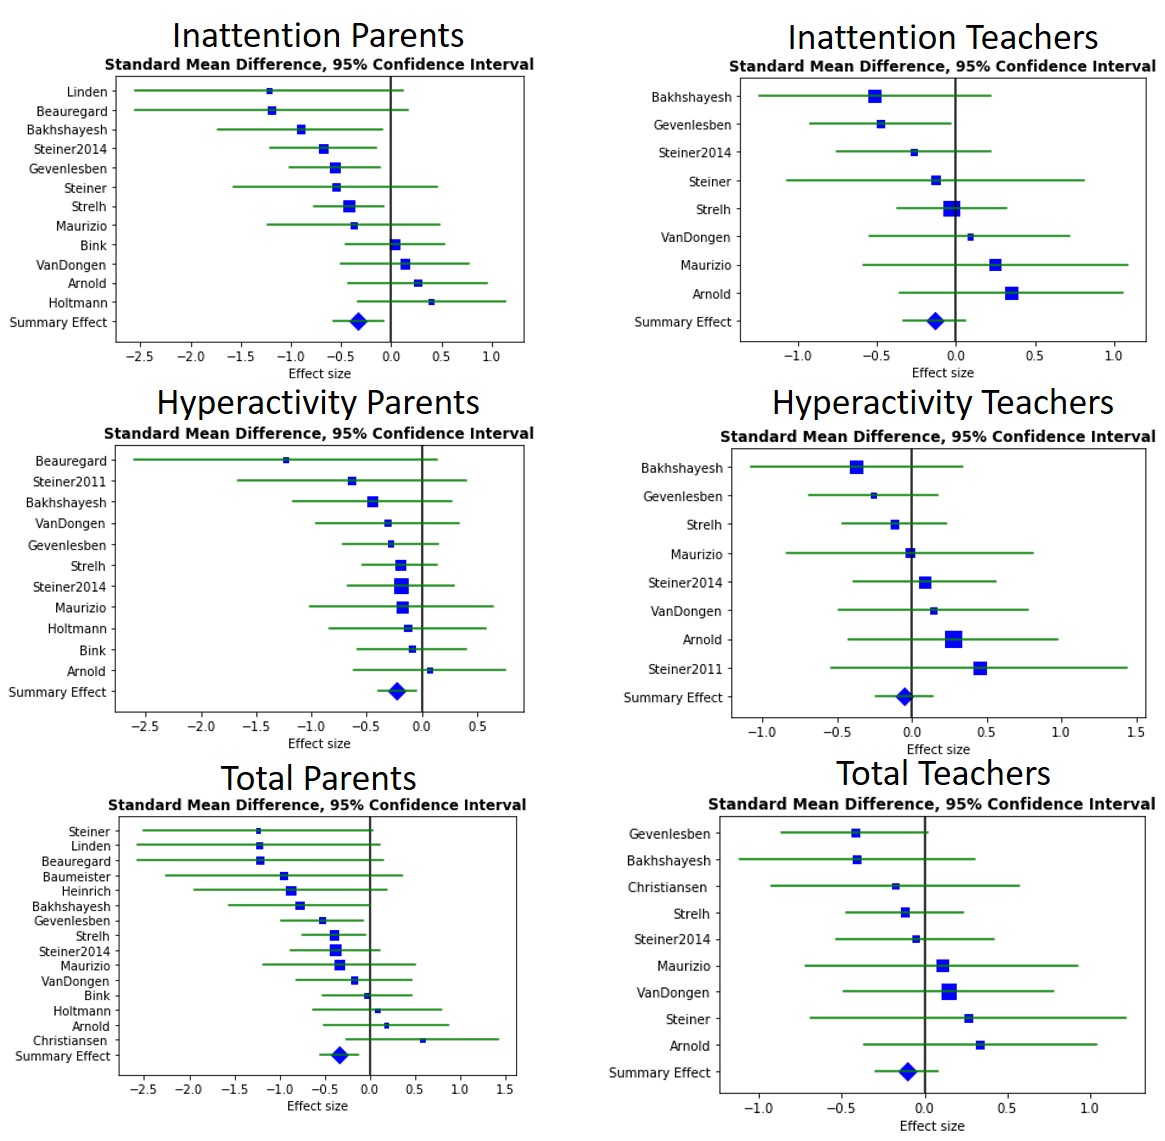
\includegraphics[width=1.0\linewidth]{figures/meta_review_forest_plots_update_meta_analysis_our_choices_no_colors_2-columns_fitting_image.jpg}
  \caption{Forest plots obtained on the dataset "Update meta-analysis" with the Python code. The \gls{es} presented here correspond to
	the between subject effect size. A negative \gls{es} is in favor of \gls{nfb}. 
	The blue squares correspond to the \gls{es}, the blue diamond to the \gls{se} and the green line to the 95\% confidence interval.}
  \label{Figure:meta_review_forest_plots_update_meta_analysis_our_choices_no_colors_2-columns_fitting_image}
\end{figure}

\begin{figure}[h!]
  \centering
  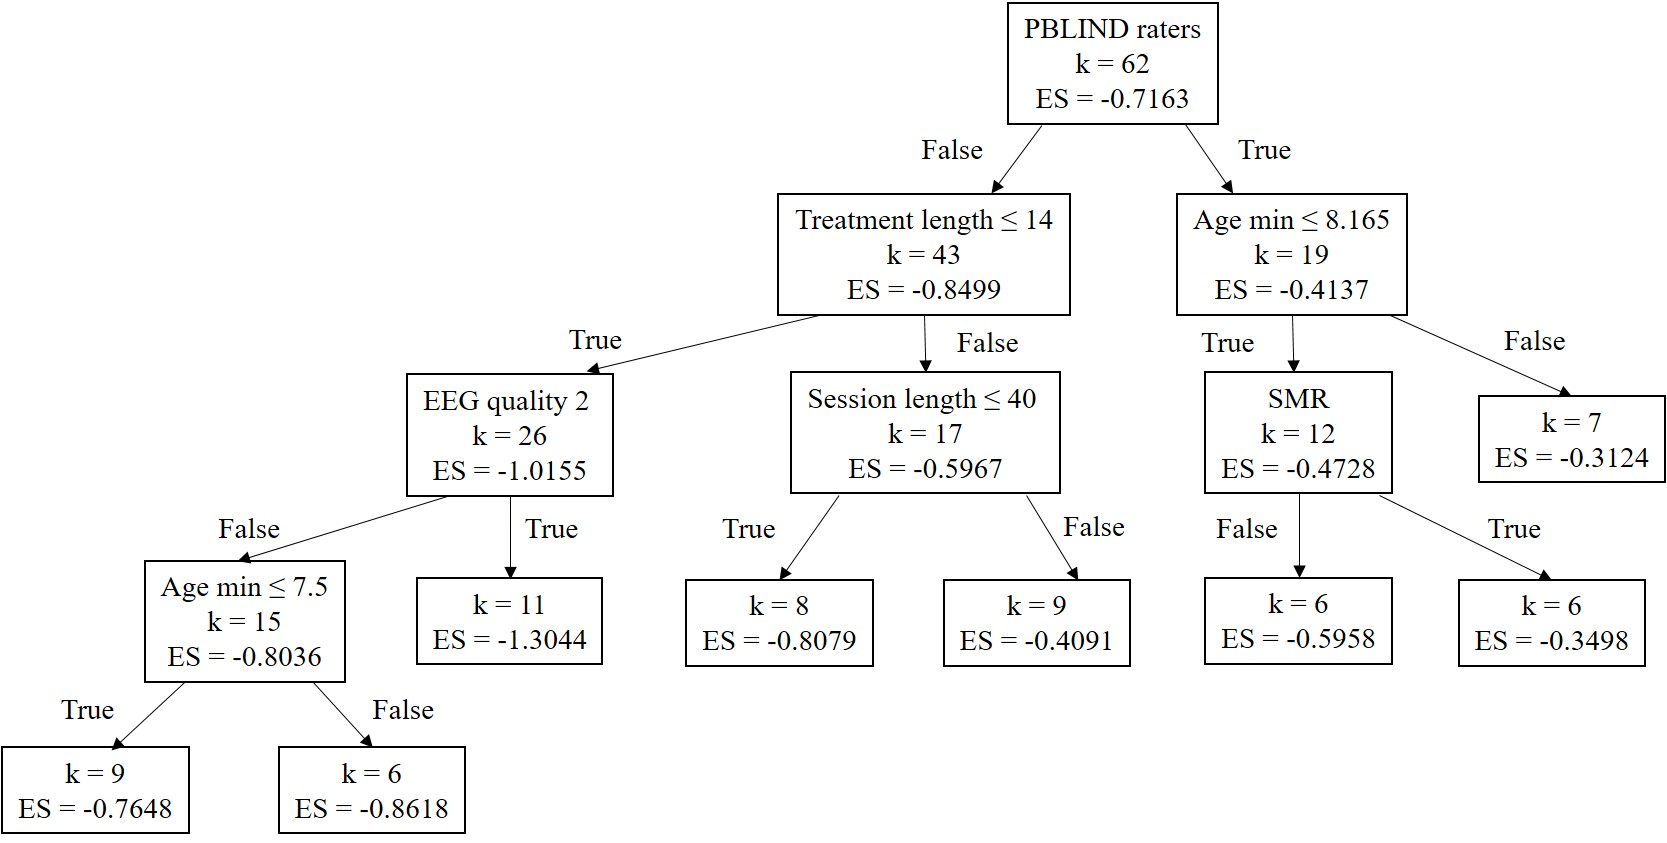
\includegraphics[width=1.0\linewidth]{figures/factors_analysis_decision_tree_results_no_colors_2-columns_fitting_image.jpg}
  \caption{Decision Tree obtained: \gls{es} corresponds to the within subject effect size and k to the number of studies. 
	The criteria to minimize was the \gls{mse}. The importance of nodes and leafs is decreasing
	from the root node.}
  \label{Figure:factors_analysis_decision_tree_results}
\end{figure}

\begin{figure}[h!]
  \centering
  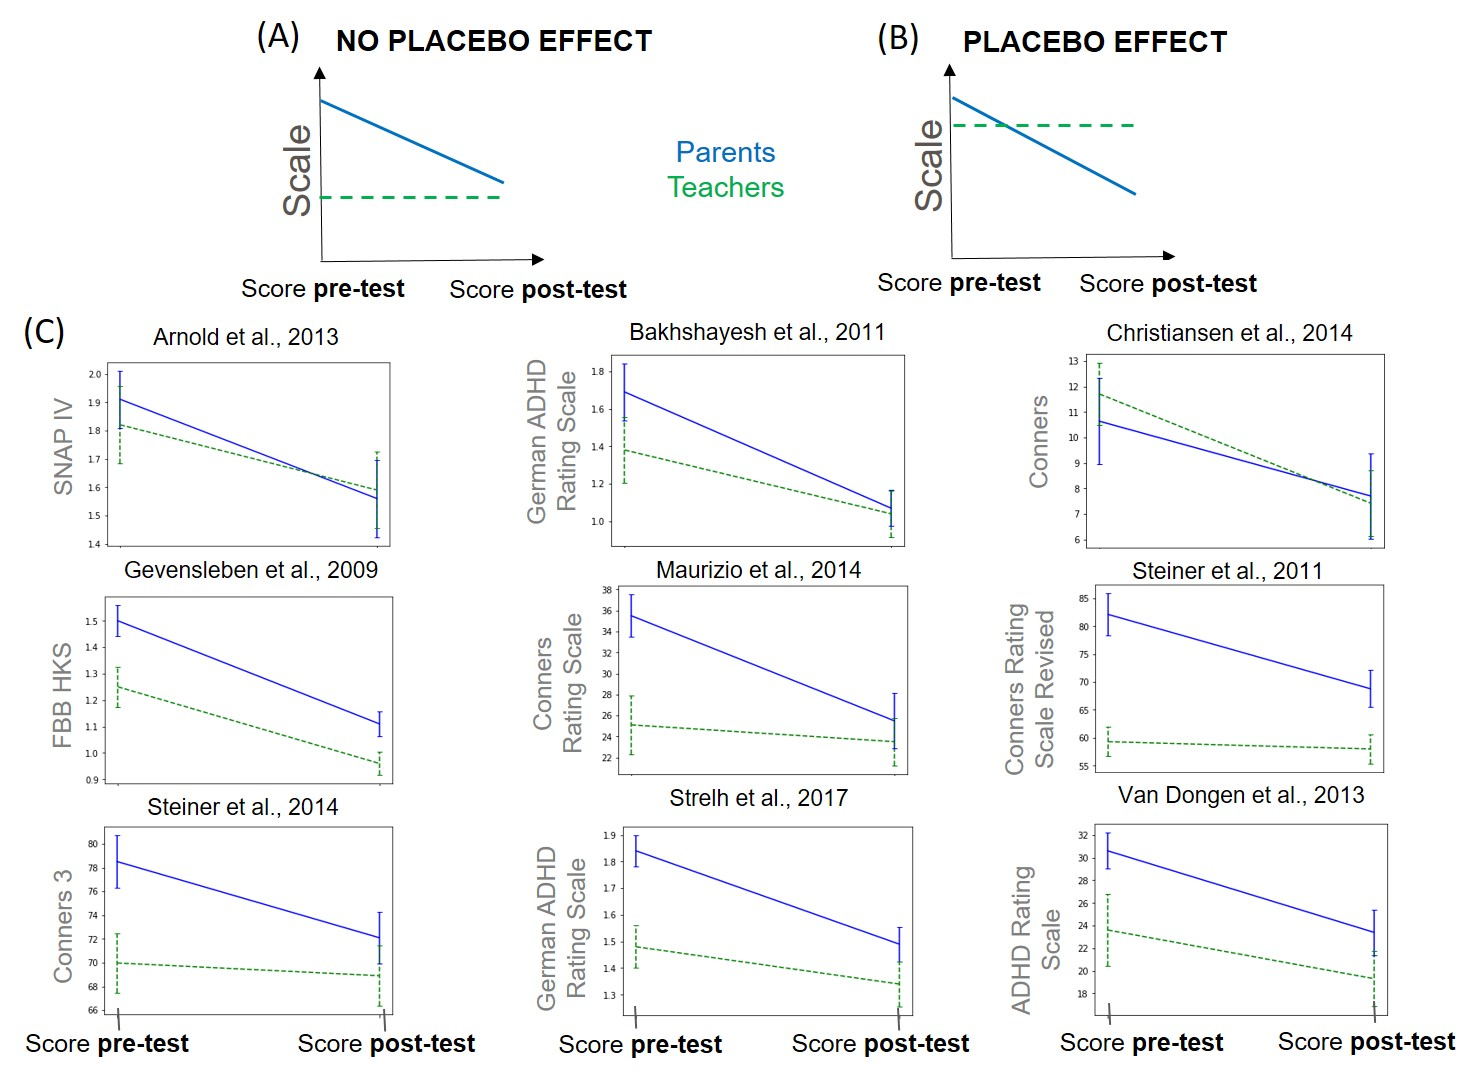
\includegraphics[width=1.0\linewidth]{figures/discussion_on_placebo_effect_colors_2-columns_fitting_image.jpg}
  \caption{Pre-test and post-test scores ($\pm$ standard error) given by Parents (\gls{mprox}) in blue and teachers (\gls{pblind}) in green. Two configurations: \textbf{(A)} teachers don’t see the symptoms at 
	pre-test so they can’t see any improvement at post-test, \textbf{(B)} teachers see the symptoms at pre-test and don’t see any improvement at post-test. \textbf{(C)} Evolution of parents and teachers' scores
	between pre and post-test on studies that satisfy \citeauthor{Cortese2016}'s inclusion criteria and that provide teachers and parents scores on the same scale.}
  \label{Figure:discussion_on_placebo_effect_colors_2-columns_fitting_image}
\end{figure} 

\clearpage

\section*{Table captions}

\begin{table}[h!]
  \centering
  \caption{List of all studies included in the three different analysis. $^a$ Studies originally included in \citet{Cortese2016}
	(search on August 30, 2015), $^b$ studies satisfying \citet{Cortese2016}'s criteria (search on December 14, 2017), $^c$ studies 
	satisfying \citet{Cortese2016}'s criteria to the exception of the part relative to the control group (search on December 14, 2017).}
  \fontsize{9}{11}\selectfont
\begin{tabular}{ cccccc }
\toprule
\multicolumn{3}{ c }{Dataset} & Study & Year & \shortstack{ Size of the \\ \gls{nfb} group } \\
\midrule
 & & & \citeauthor{Arnold2014} & 2014 & 26 \\ 
 & & & \citeauthor{Bakhshayesh2011} & 2011 & 18 \\
 & & & \citeauthor{Beauregard2006} & 2006 & 15 \\
 & & & \citeauthor{Bink2014} & 2014 & 45 \\
 & & & \citeauthor{Christiansen2014} & 2014 & 14 \\
 & & & \citeauthor{Gevensleben2009} & 2009 & 59 \\
 & & & \citeauthor{Heinrich2004} & 2004 & 13 \\
 & & & \citeauthor{Holtmann2009} & 2009 & 20 \\
 & & & \citeauthor{Linden1996} & 1996 & 9 \\
 & & & \citeauthor{Maurizio2014} & 2014 & 13 \\
 & & & \citeauthor{Steiner2011} & 2011 & 9 \\
 & & & \citeauthor{Steiner2014} & 2014 & 34 \\
 & & |\shortstack{ Replicate \\ \citeauthor{Cortese2016}$^a$ } & \citeauthor{VanDongen2013} & 2013 & 22 \\
\cmidrule(lr){3-6}
 & & & \citeauthor{Baumeister2016} & 2016 & 8 \\
 & \shortstack{ Update \\ \citeauthor{Cortese2016}$^b$ } & & \citeauthor{Strehl2017} & 2017 & 72 \\
\cmidrule(lr){2-6}
 & & & \citeauthor{Bluschke2016} & 2016 & 19 \\
 & & & \citeauthor{Deilami2016} & 2016 & 12 \\
 & & & \citeauthor{Drechsler2007} & 2007 & 17 \\
 & & & \citeauthor{Duric2012} & 2012 & 23 \\
 & & &\citeauthor{Escolano2014} & 2014 & 20 \\
 & & & \citeauthor{Fuchs2003} & 2003 & 22 \\
 & & & \citeauthor{Kropotov2005} & 2005 & 86 \\
 & & & \citeauthor{Lee2017} & 2017 & 18 \\
 & & & \citeauthor{Leins2007} & 2007 & 19 \\
 & & & \citeauthor{Li2013} & 2013 & 20 \\
 & & & \citeauthor{Meisel2014} & 2014 & 12 \\
 & & & \citeauthor{Mohagheghi2017} & 2017 & 30 \\
 & & & \citeauthor{Mohammadi2015} & 2015 & 16 \\
 & & & \citeauthor{Monastra2002} & 2002 & 51 \\
 & & & \citeauthor{Ogrim2013} & 2013 & 13 \\
 \gls{saob}$^c$ & & & \citeauthor{Strehl2006} & 2006 & 23 \\
\bottomrule
\end{tabular}

  \label{Table:table_factors_analysis_meta_analysis_list_studies}
\end{table}

\begin{table}[h!]
  \centering
  \caption{Comparison between \citet{Cortese2016} results obtained with RevMan \citep{RevMan} and those obtained with the Python code with our 
	choices applied ($^a$ post-test values for \citeauthor{Arnold2014} are obtained after 40 sessions of \gls{nfb} and Conners scale is used for \citeauthor{Steiner2014}
	teachers' outcomes). \glspl{se} and their corresponding p-value (in parenthesis) are presented. With the Python program, a negative \gls{se}
	is in favor of \gls{nfb} unlike \citeauthor{Cortese2016}.}
\begin{tabular}{cccc}

\toprule
\multicolumn{2}{c}{Input data} & \shortstack{ Results from \\ \citet{Cortese2016} \\ (for reference)} & \shortstack{ Means and standard \\ deviations from \\ articles included in \\ \citet{Cortese2016} }\\
\midrule
\multicolumn{2}{c}{Implementation} & \shortstack{ RevMan \\ \citet{RevMan} } & Python program\\
\midrule
\multicolumn{2}{ c }{Hypothesis} & \shortstack{ Same as \\ \citet{Cortese2016} } & Our choices$^a$\\
\midrule
\multirow{ 3}{*}{ \textit{Parents} } & Total & $0.35$ ($0.004$) & $-0.32$ ($0.013$)\\
 & Inattention  & $0.36$ ($0.009$) & $-0.31$ ($0.036$)\\
 & Hyperactivity  & $0.26$ ($0.004$) & $-0.24$ ($0.02$)\\
\multirow{ 3}{*}{ \textit{Teachers} } & Total & $0.15$ ($0.20$) & $-0.11$ ($0.37$)\\
 & Inattention  & $0.06$ ($0.70$) & $-0.17$ ($0.16$)\\
 & Hyperactivity  & $0.17$ ($0.13$) & $-0.022$ ($0.85$)\\
\bottomrule

\end{tabular}

  \label{Table:meta_review_comparison_revman_and_python_with_choices}
\end{table}

\begin{table}[h!]
  \centering
  \caption{Results of the \gls{wls}, \gls{lasso} and decision tree. For the \gls{wls}, a p-value $<$ 0.05 (in bold) means that the coefficient of 
	the corresponding factor is significantly different from 0. For the \gls{lasso}, factors not set to 0 (in bold) are selected. For the decision tree,
	the place of the factor in the tree is precised. When the value of the coefficient is negative, the corresponding factor may lead to better \gls{nfb} results.}
  \begin{center}
\begin{tabular}{ p{3cm} p{3cm} p{3cm} p{2cm} p{2cm} p{2cm}}
\toprule
\multicolumn{2}{c}{ \shortstack{Independent \\ variables (factors)} } & \shortstack{ \gls{wls} \\ (p-value) } & \gls{lasso} & \shortstack{Decision \\ Tree} \\
\midrule
\multirow{ 2}{*}{ \textit{Signal quality} } & \gls{eog} correction & \hskip 0.08in-0.078 (0.41) &  \hskip 0.12in0.00 & / \\ 
& artifact correction based on amplitude & \hskip 0.12in\textbf{0.15(0.040)} & \hskip 0.12in\textbf{0.047} & / \\ 
\midrule
\multirow{ 3}{*}{ \textit{Methodological} } & \gls{pblind} & \hskip 0.12in\textbf{0.10 (0.043)} & \hskip 0.12in\textbf{0.11} & \textbf{selected} \\ 
& randomization & \hskip 0.12in0.0069 (0.92) & \hskip 0.12in\textbf{0.032} & / \\  
& \gls{irb} & \hskip 0.08in\textbf{-0.29 (0.00)} & \hskip 0.08in\textbf{-0.15} & / \\  
\midrule
\multirow{ 3}{*}{ \textit{Population} } & age max & \hskip 0.08in-0.090 (0.16) & \hskip 0.12in0.00 & / \\
& age min & \hskip 0.08in-0.055 (0.37) & \hskip 0.12in0.00 & \textbf{selected }\\
& on drugs & \hskip 0.12in0.069 (0.42) & \hskip 0.12in\textbf{0.032} & / \\
\midrule
\multirow{ 9}{*}{ \textit{ \shortstack{\gls{nfb} \\ implementation} } } & number of sessions  & \hskip 0.08in-0.0075 (0.92) & \hskip 0.12in0.00 & / \\
& session length & \hskip 0.12in0.17 (0.17) & \hskip 0.12in0.00 & \textbf{selected} \\
& treatment length & \hskip 0.12in\textbf{0.57 (0.00)} & \hskip 0.12in\textbf{0.33} & \textbf{selected} \\
& session pace & \hskip 0.08in\textbf{-0.25 (0.00)} & \hskip 0.08in\textbf{-0.14} & / \\ 
& \gls{smr} & \hskip 0.08in-0.063 (0.41) & \hskip 0.12in\textbf{0.061} & \textbf{selected} \\
& beta up central & \hskip 0.08in-0.027 (0.72) & \hskip 0.12in0.00 & / \\  
& theta down & \hskip 0.08in\textbf{-0.29 (0.014)} & \hskip 0.08in\textbf{-0.051} & / \\
& \gls{scp} & \hskip 0.08in-0.099 (0.50) & \hskip 0.12in\textbf{0.10} & / \\ 
& transfer phase & \hskip 0.12in\textbf{0.27 (0.032)} & \hskip 0.12in\textbf{0.11} & / \\
\midrule
\multirow{ 2}{*}{ \textit{ \shortstack{Quality of \\ acquisition} } } & more than one active electrode & \hskip 0.12in0.064 (0.36) & \hskip 0.12in0.00 & / \\ 
& \gls{eeg} quality 2 & \hskip 0.08in\textbf{-0.36 (0.00)} & \hskip 0.08in\textbf{-0.23} & \textbf{selected} \\  
\bottomrule
\end{tabular}
\end{center}

  \label{Table:table_factors_analysis_results_summary}
\end{table}

\end{document}